\documentclass{beamer}
\mode<presentation>{
\usetheme{Madrid}
%\setbeamertemplate{caption}[numbered]
%\setbeamertemplate{footline} % To remove the footer line in all slides uncomment this line
\setbeamertemplate{footline}[page number] % To replace the footer line in all slides with a simple slide count uncomment this line
\setbeamertemplate{navigation symbols}{}
}

\usepackage{amsmath}
\usepackage{graphicx}
\usepackage{mathtools}
\usepackage[font={scriptsize}]{caption}

\title[Ruido en circuitos gen\'eticos]{Modelos de ruido intr\'inseco en circuitos gen\'eticos}
\author{Luis Alberto Guti\'errez L\'opez}
\institute[Uniandes]{Universidad de los Andes\\
Departamento de F\'isica\\
Seminario de Biof\'isica
\medskip
}
\date{Septiembre 1 de 2015}

\begin{document}

\begin{frame}
\titlepage
\end{frame}

\begin{frame}
\frametitle{Introducci\'on}
\begin{itemize}
\item Fluctuaciones aleatorias en expresi\'on gen\'etica.
\item En transcripci\'on y traducci\'on: Colisiones aleatorias entre mol\'eculas que se encuentran en bajo n\'umero.
\item Otros factores como la divisi\'on celular, la disposici\'on de los organelos, la variablidad del ambiente y el ciclo celular.
\begin{align*}
\eta_X &= \frac{\sigma_X}{\langle X \rangle}.\\[1.5ex]
\nu_X &= \frac{\sigma^2_X}{\langle X \rangle}.
\end{align*}
\end{itemize}
\end{frame}


\begin{frame}
\begin{figure}[p]
    \centering
    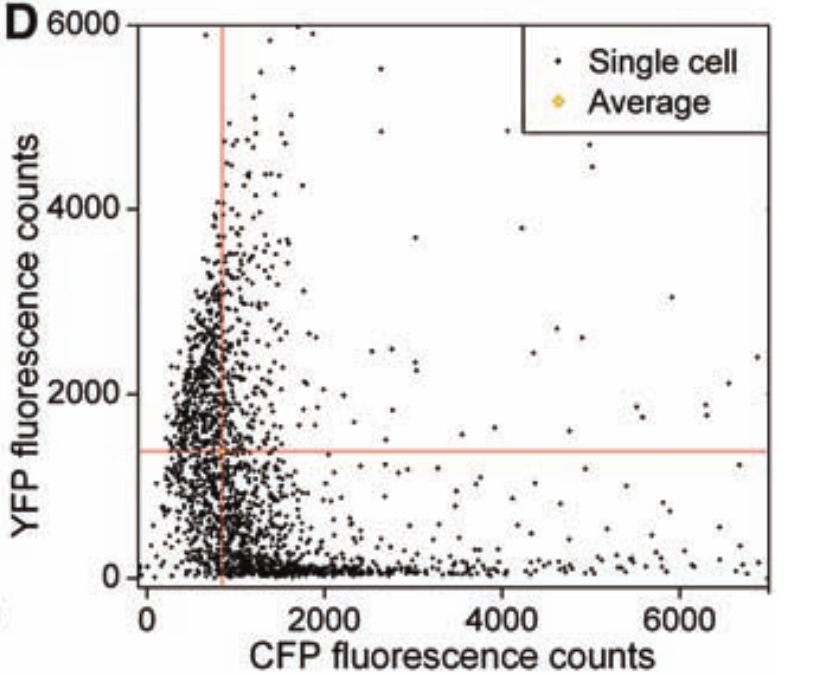
\includegraphics[width=0.5\textwidth]{noiseGFP.png}\\
    \tiny \cite{p3}.
    \label{1}
\end{figure}
\end{frame}


\begin{frame}
\hspace{20 mm} \textbf{Robustez} \hspace{40 mm} \textbf{Variabilidad}
\begin{columns}[c]
\column{.5\textwidth}
\begin{figure}[p]
    \centering
    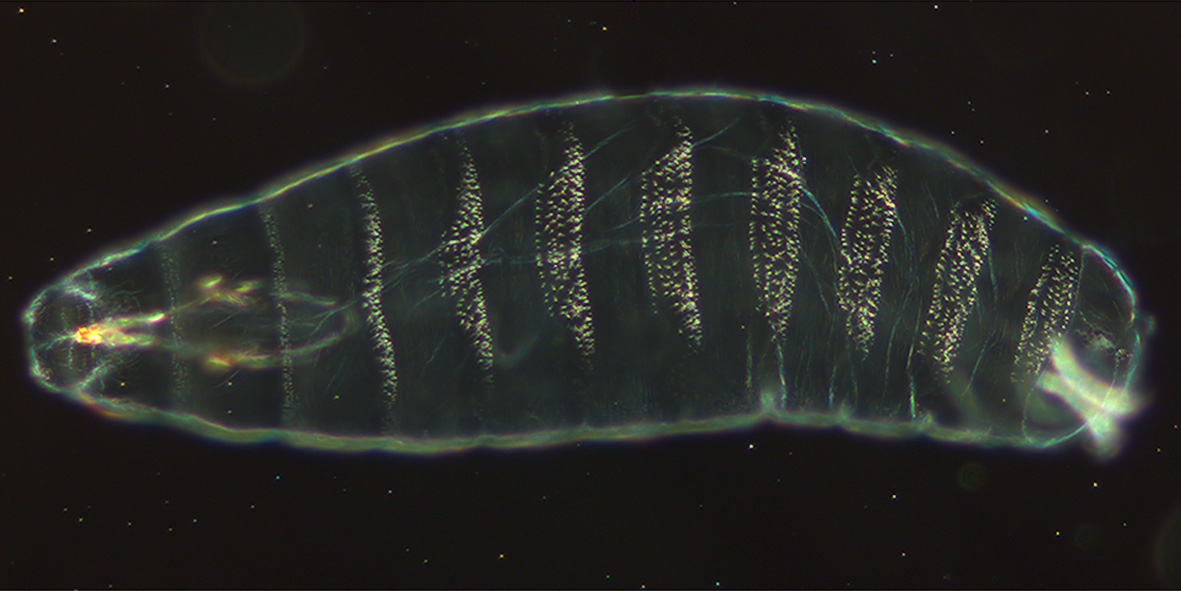
\includegraphics[width=0.9\textwidth]{drosophila.jpg}\\
    \tiny Tomado de: \url{https://en.wikipedia.org/wiki/Drosophila_embryogenesis}.
\end{figure}

\column{.5\textwidth}
\begin{figure}[p]
    \centering
    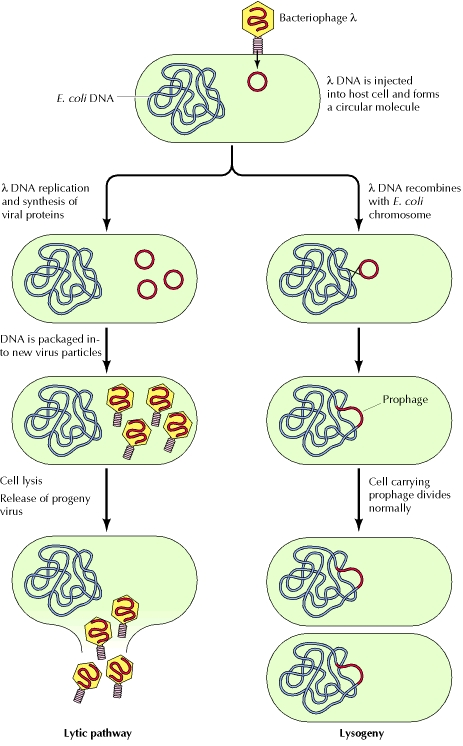
\includegraphics[width=0.7\textwidth]{lambda.jpg}\\
    \tiny \cite{p4}.
\end{figure}
\end{columns}
\end{frame}


%\begin{frame}
%\begin{figure}[p]
%    \centering
%    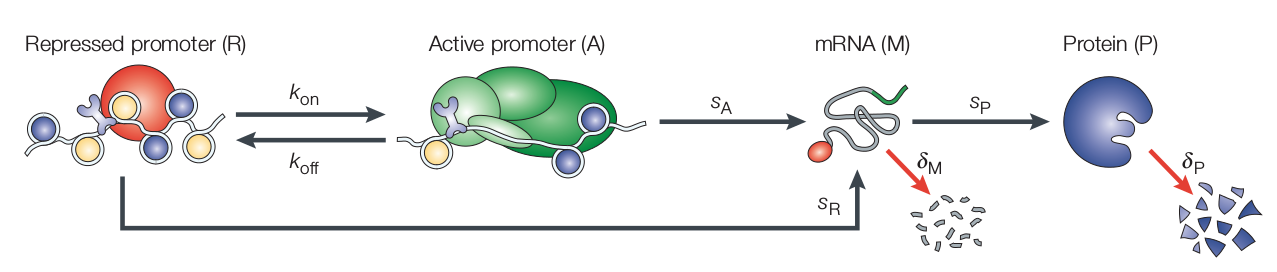
\includegraphics[width=1\textwidth]{expression.png}\\
%    \tiny \cite{p2}.
%\end{figure}
%\end{frame}

\begin{frame}
\begin{figure}[p]
    \centering
    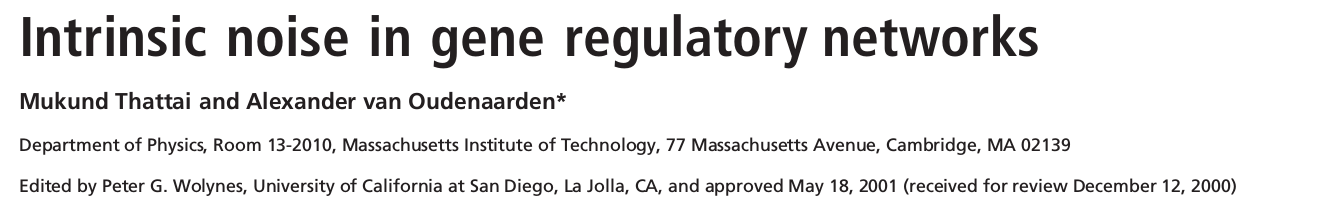
\includegraphics[width=1\textwidth]{title.png}\\
    \tiny \cite{p1}.
\end{figure}
\end{frame}

\begin{frame}
\frametitle{Suposiciones}
\begin{columns}[c]
\column{0.5\textwidth}
\begin{itemize}
\item Las interacciones con factores de transcripci\'on se consideran en equilibrio.
\item La tasa de producci\'on de ARN es cte., as\'i como la de producci\'on de prote\'inas por cada ARN.
\item Los ribosomas se pueden unir al RNA casi inmediatamente inicia la transcripci\'on.
\item Tasas de decaimiento $\gamma_R$ y $\gamma_P$.
\end{itemize}
\column{0.4\textwidth}
\begin{figure}[p]
    \centering
    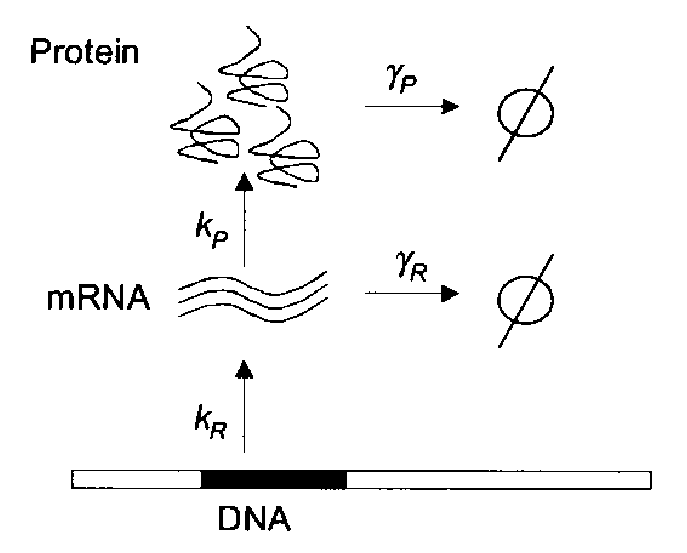
\includegraphics[width=1\textwidth]{expressionsimple.png}\\
    \tiny \cite{p1}.
\end{figure}
\centering \textbf{Ecuaciones deterministas}
\begin{align*}
\dot{r}(t) &= k_R - \gamma_Rr(t).\\
\dot{p}(t) &= k_Pr(t) - \gamma_Pp(t).
\end{align*}
\end{columns}
\end{frame}


%\begin{frame}
%\frametitle{Un s\'olo gen - Modelo}
%\begin{figure}[p]
%    \centering
%    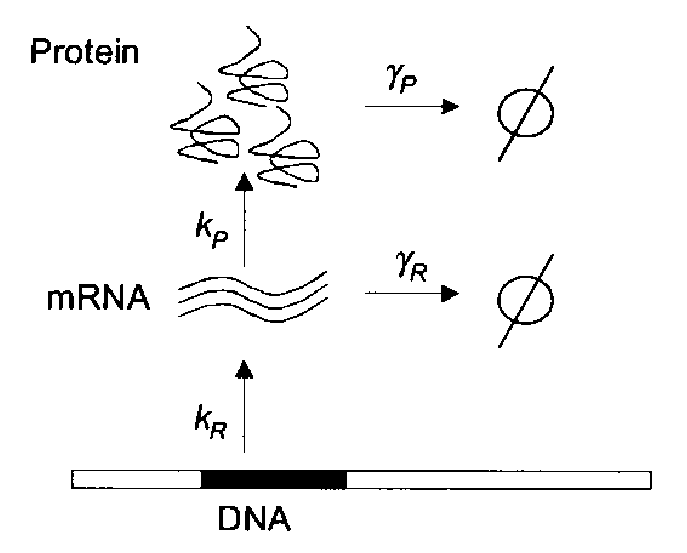
\includegraphics[width=0.4\textwidth]{expressionsimple.png}\\
%    \tiny \cite{p1}.
%\end{figure}
%\centering \textbf{Ecuaciones deterministas}
%\begin{align*}
%\dot{r}(t) &= k_R - \gamma_Rr(t).\\
%\dot{p}(t) &= k_Pr(t) - \gamma_Pp(t).
%\end{align*}
%\end{frame}

\begin{frame}
\begin{figure}[p]
    \centering
    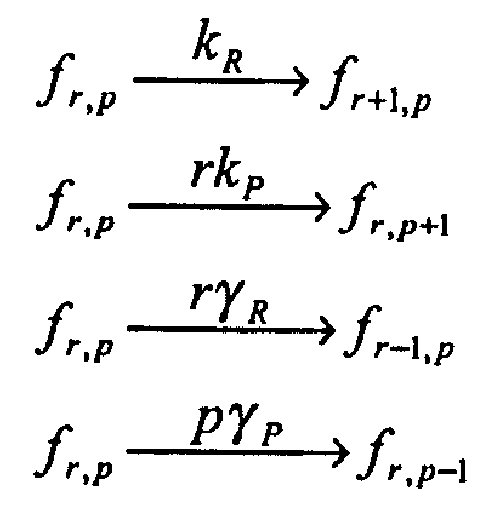
\includegraphics[width=0.3\textwidth]{scheme1.png}\\
    \tiny \cite{p1}.
\end{figure}
\centering \textbf{Ecuaci\'on maestra}
\begin{align*}
\frac{d{f}_{r,p}}{dt} &= k_Rf_{r-1,p} - k_Rf_{r,p} + k_Prf_{r,p-1} - k_Prf_{r,p}\\
&+ \gamma_R(r+1)f_{r+1,p} - \gamma_Rrf_{r,p} + \gamma_P(p+1)f_{r,p+1} - \gamma_Ppf_{r,p}.
\end{align*}
\end{frame}

\begin{frame}
\frametitle{Un s\'olo gen - Resultados}

\begin{columns}[c]
\column{.45\textwidth}
\centering \textbf{Promedio}
\begin{align*}
\langle r \rangle &= \frac{k_R}{\gamma_R}.\\[1.5ex]
\langle p \rangle &= \frac{k_Rb}{\gamma_P}.
\end{align*}
\column{.5\textwidth}
\centering \textbf{Ruido}
\begin{align*}
\nu_r &= \frac{\sigma_r^2}{\langle r \rangle} = 1.\\[1.5ex]
\nu_p &= \frac{\sigma_p^2}{\langle p \rangle} = \frac{b}{1+\eta} + 1 \approx b + 1.
\end{align*}
\end{columns}

\vspace{3 mm}

\begin{equation*}
b \coloneqq \frac{k_P}{\gamma_R}, \quad \eta \coloneqq \frac{\gamma_P}{\gamma_R}.
\end{equation*}

\end{frame}

\begin{frame}
\begin{figure}[p]
    \centering
    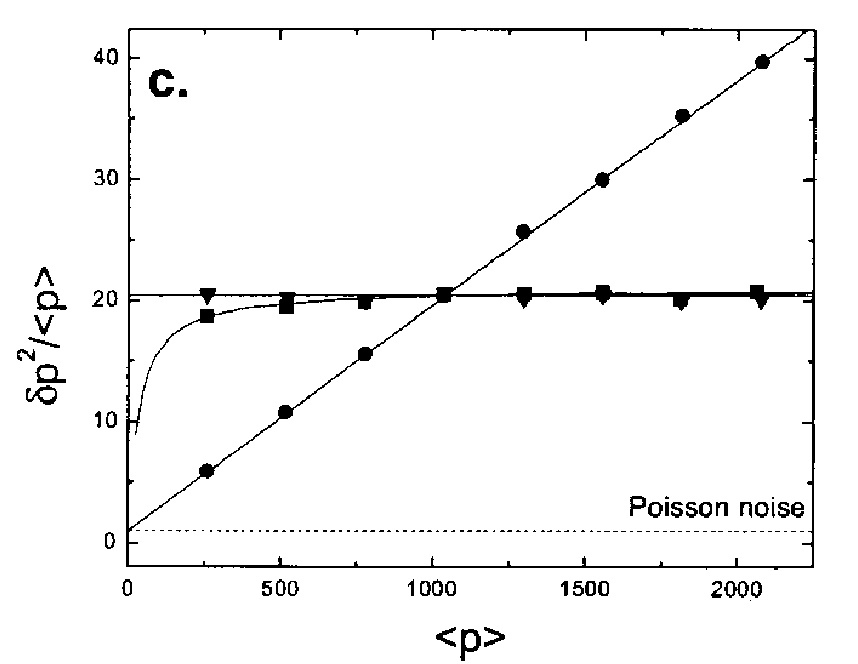
\includegraphics[width=0.6\textwidth]{graph1.png}\\
    \tiny \cite{p1}.
    \caption{C\'irculos: var\'ia $b$. Tri\'angulos: var\'ia $k_R$. Cuadros: var\'ia $\gamma_R$. L\'inea s\'olida: ecuaciones. S\'imbolos: simulaciones.}
\end{figure}
\begin{equation*}
\nu_p = \frac{b}{1+\eta} + 1 \approx b + 1; \quad b = \frac{k_P}{\gamma_R}, \quad \eta = \frac{\gamma_P}{\gamma_R}.
\end{equation*}
\end{frame}


\begin{frame}
\frametitle{Generalizaci\'on}

Las ecuaciones

\begin{align*}
\dot{r}(t) &= k_r - \gamma_rr(t),\\
\dot{p}(t) &= k_pr(t) - \gamma_pp(t),
\end{align*}

pueden ser escritas como

\begin{equation*}
\mathbf{\dot{x}} = (A - \Gamma)\mathbf{x}.
\end{equation*}

Donde $\mathbf{x}^T \coloneqq (d, r, p)$ y

\begin{align*}
A \coloneqq \bordermatrix{
  ~ & (d) & (r) & (p) \cr
  (d) & 0 & 0 & 0 \cr
  (r) & k_R & 0 & 0 \cr
  (p) & 0 & k_P & 0 \cr}, \quad \quad
\Gamma \coloneqq \bordermatrix{
  ~ & (d) & (r) & (p) \cr
  (d) & 0 & 0 & 0 \cr
  (r) & 0 & \gamma_R & 0 \cr
  (p) & 0 & 0 & \gamma_P \cr}.\\
\end{align*}
\end{frame}

\begin{frame}
Se puede realizar en general. Si $\mathbf{x}^T \coloneqq (q_1,q_2,\dots,q_n)$, 
\begin{figure}[p]
    \centering
    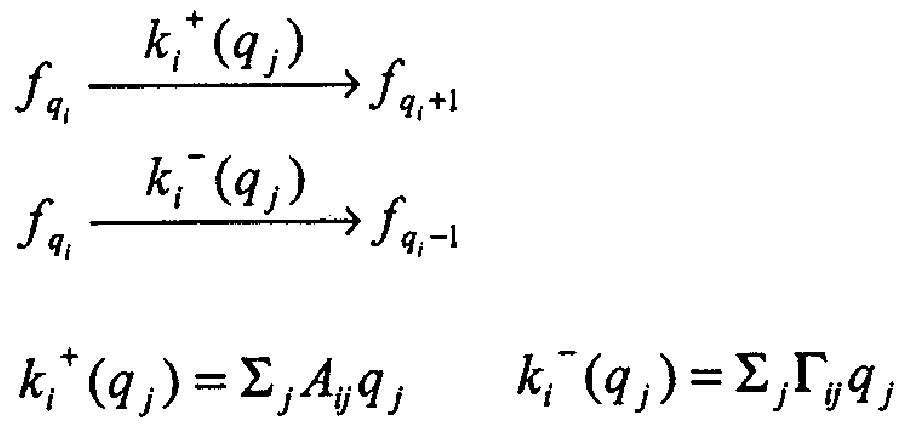
\includegraphics[width=0.6\textwidth]{scheme2.png}\\
    \tiny \cite{p1}.
\end{figure}
la ecuaci\'on maestra queda
\begin{equation*}
\dot{f}_{q_i} = \sum_j \left[\left(A_{ij}q_j\right) \left(f_{q_{i-1}} - f_{q_i}\right)\right] + \Gamma_{ii}q_{i+1}f_{q_{i+1}} -\Gamma_{ii}q_if_{q_i}.
\end{equation*}
\end{frame}

\begin{frame}
\frametitle{Autorregulaci\'on - Modelo}
\begin{figure}[p]
    \centering
    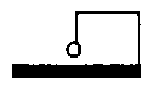
\includegraphics[width=0.2\textwidth]{autorreg.png}\\
    \tiny \cite{p1}.
\end{figure}
\begin{columns}[c]

\column{.5\textwidth}
\begin{figure}[p]
    \centering
    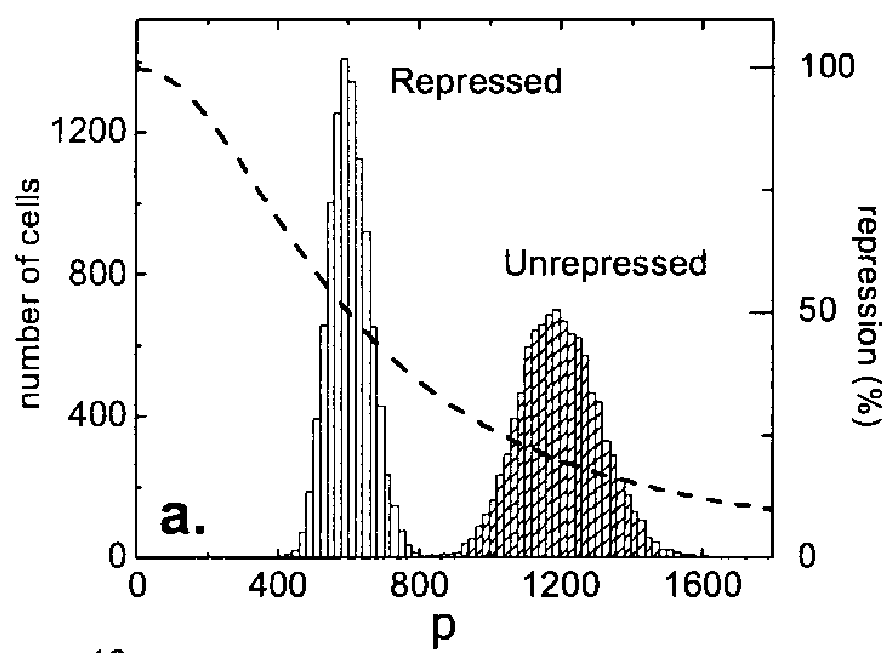
\includegraphics[width=1\textwidth]{graph3.png}\\
    \tiny \cite{p1}.
\end{figure}

\column{.5\textwidth}
\begin{itemize}
\item Ecuaci\'on de Hill.
\begin{equation*}
k_R = \frac{k_R^{\text{max}}}{1+(p/K_d)^n}.
\end{equation*}
\item Linearizar alrededor del promedio en estado estacionario.
\begin{equation*}
k_R \approx k_0-k_1p.
\end{equation*}
\begin{equation*}
A = 
\begin{pmatrix}
0 & 0 & 0 \\
k_0 & 0 & -k_1 \\
0 & k_P & 0
\end{pmatrix}.
\end{equation*}
\end{itemize}
\end{columns}
\end{frame}

\begin{frame}
\frametitle{Autorregulaci\'on - Resultados}
\begin{columns}[c]

\column{.45\textwidth}
\centering \textbf{Promedio}
\begin{align*}
%\langle r \rangle &= .\\[1.5ex]
\langle p \rangle &= \frac{1}{1+b\phi} \cdot \frac{k_0b}{\gamma_p}.
\end{align*}

\column{.5\textwidth}
\centering \textbf{Ruido}
\begin{align*}
%\nu_r &= .\\[1.5ex]
\nu_p &= \frac{1-\phi}{1+b\phi} \cdot \frac{b}{1+\eta}+1.
\end{align*}
\end{columns}

\vspace{3 mm}

\begin{equation*}
  b \coloneqq \frac{k_P}{\gamma_R}, \quad \eta \coloneqq \frac{\gamma_P}{\gamma_R}, \quad \phi \coloneqq \frac{k_1}{\gamma_P}.
\end{equation*}

\begin{figure}[p]
    \centering
    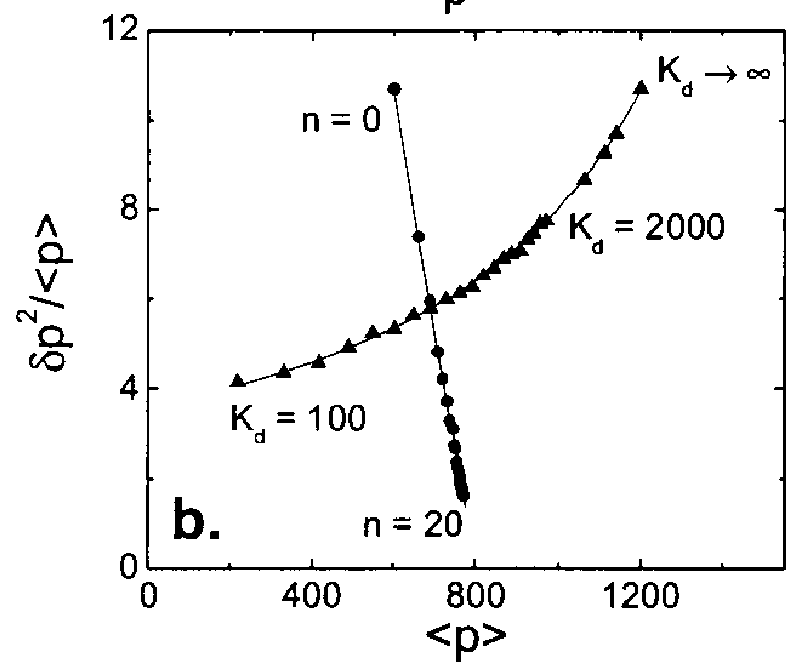
\includegraphics[width=0.5\textwidth]{graph5.png}\\
    \tiny \cite{p1}.
\end{figure}

\end{frame}


\begin{frame}
\frametitle{En general}
\begin{columns}[c]
\column{.6\textwidth}
\begin{figure}[p]
    \centering
    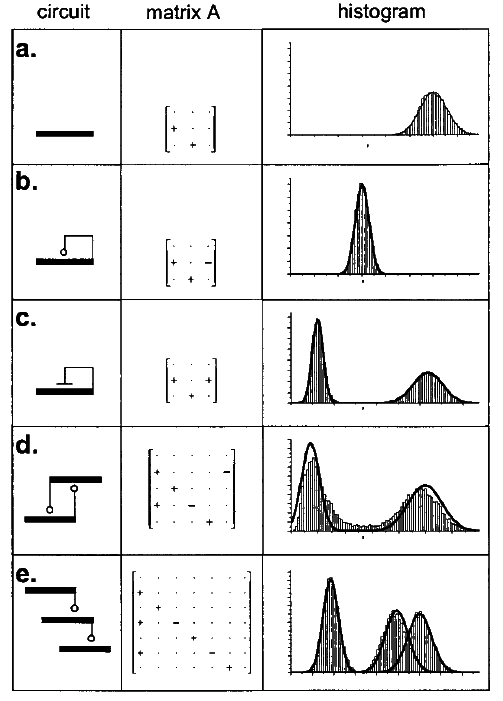
\includegraphics[width=0.75\textwidth]{graph4.png}\\
    \tiny \cite{p1}.
\end{figure}
\column{.4\textwidth}
\begin{itemize}
\item Posibilidad de biestabilidad.
\item Linearizar alrededor de cada punto de equilibrio.
\end{itemize}
\end{columns}
\end{frame}

\begin{frame}
\frametitle{Problemas}
\begin{itemize}
\item Hay muchas otras fuentes de ruido que no se consideran.
\item Modelo linearizado.
%\item Otros tipos de reacciones pueden afectar el ruido del sistema.
\item No sirve para explicar el comportamiento lejos de los puntos fijos si el sistema es no lineal.
\end{itemize}
\end{frame}

\begin{frame}
\frametitle{Referencias}
\footnotesize{
\begin{thebibliography}{99}

\bibitem[Thattai \& van Oudenaarden, 2001]{p1} Thattai, M. \& van Oudenaarden, A. (2001).
\newblock Intrinsic noise in gene regulatory networks.
\newblock \emph{PNAS} 98(15), 8614 -- 8619.

\bibitem[Kaern et al., 2012]{p2} Kaern, M., Elston, T. C., Blake, W. J. \& Collins, J. J. (2005).
\newblock Stochasticity in gene expression: from theories to phenothypes.
\newblock \emph{Nat Rev Genet} 6(6), 451 -- 464.

\bibitem[Pedraza \& van Oudenaarden, 2005]{p3} Pedraza, J. M. \& van Oudenaarden, A. (2005).
\newblock Noise Propagation in Gene Networks.
\newblock \emph{Science} 307, 1965 -- 1969.

\bibitem[Cooper, 2000]{p4} Cooper, G. M. (2000).
\newblock The Cell, A Molecular Approach. 2nd Edition.
\newblock Sunderland (MA): Sinauer Associates.
\end{thebibliography}
}
\end{frame}

\end{document}
